\section{Descripción de proceso}

Como se introdujo en el Capítulo \ref{chpt:intro}, un \textbf{proceso} puede definirse como un programa en ejecución. Más precisamente, es la entidad que el sistema operativo administra y asigna al procesador para su ejecución. Un proceso está compuesto por el código del programa, los datos asociados y toda la información necesaria para describir su estado de ejecución.

Cada proceso se caracteriza por un conjunto de atributos, entre los que destacan:
\begin{itemize}
  \item Un identificador único (PID).
  \item Su estado de ejecución.
  \item Su prioridad.
  \item El contador de programa (Program Counter, PC).
  \item Los punteros a las regiones de memoria que utiliza.
  \item El contexto del procesador (contenido de los registros).
  \item Información sobre operaciones de entrada/salida y archivos abiertos.
  \item Información administrativa, como el tiempo de CPU consumido o los recursos asignados.
\end{itemize}

Toda esta información se almacena en una estructura denominada \textbf{Bloque de Control de Proceso} (\emph{Process Control Block}, PCB), creada y administrada por el sistema operativo. El PCB contiene toda la información necesaria para suspender un proceso y reanudar posteriormente su ejecución sin alterar su funcionamiento. Para ello, cuando ocurre una interrupción o un cambio de contexto, el sistema operativo guarda en el PCB el estado actual del proceso y restaura el estado del siguiente proceso que será ejecutado.

En consecuencia, un proceso puede entenderse como la combinación del programa, sus datos y el correspondiente PCB. Esta estructura constituye la base que permite al sistema operativo ejecutar múltiples procesos de forma concurrente mediante la planificación y el cambio de contexto.

\section{Estados de un proceso}

Cuando un programa se ejecuta, el sistema operativo crea un proceso para representarlo. Su ejecución puede analizarse desde dos puntos de vista:
\begin{itemize}
  \item Desde el punto de vista del programa, un proceso ejecuta una secuencia de instrucciones pertenecientes únicamente a ese programa. Esta secuencia recibe el nombre de traza (trace) del proceso.
  \item Desde el punto de vista del procesador, este ejecuta instrucciones de distintos procesos de forma alternada. El contador de programa cambia entre procesos según las decisiones del sistema operativo, por lo que las trazas de los distintos procesos aparecen intercaladas.
\end{itemize}
Como ejemplo, supóngase que existen tres procesos, A, B y C como muestra la figura \ref{fig:traza_procesos}, completamente cargados en memoria principal, además de un pequeño dispatcher (o activador) encargado de realizar el cambio de contexto entre procesos.

\begin{figure}[!ht]
  \centering
  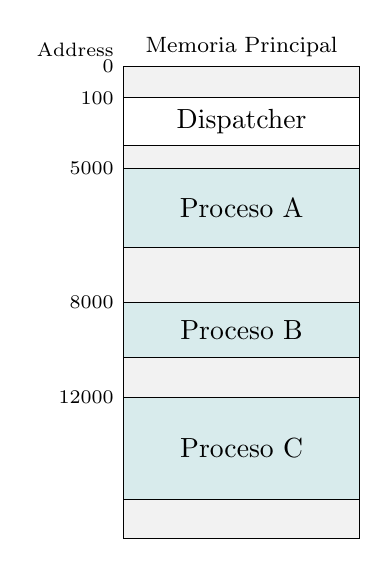
\begin{tikzpicture}
    \draw[fill=gray!10] (0,0) rectangle (3,6);
    \draw[fill=white] (0,5) rectangle node[align=center]{Dispatcher} (3,5.6);
    \draw[fill=white!92!green!92!blue] (0,3.7) rectangle node[align=center]{Proceso A} (3,4.7);
    \draw[fill=white!92!green!92!blue] (0,2.3) rectangle node[align=center]{Proceso B} (3,3);
    \draw[fill=white!92!green!92!blue] (0,0.5) rectangle node[align=center]{Proceso C} (3,1.8);
    \foreach \y\i in {1.8/12000,3/8000,4.7/5000,5.6/100,6/0} {
      \node[font=\scriptsize,left] at (0,\y) {\i};
    }
    \node[above left,font=\scriptsize] at (0,6) {Address};
    \node[above,font=\footnotesize] at (1.5,6) {Memoria Principal};
  \end{tikzpicture}
  \hspace{1cm}
  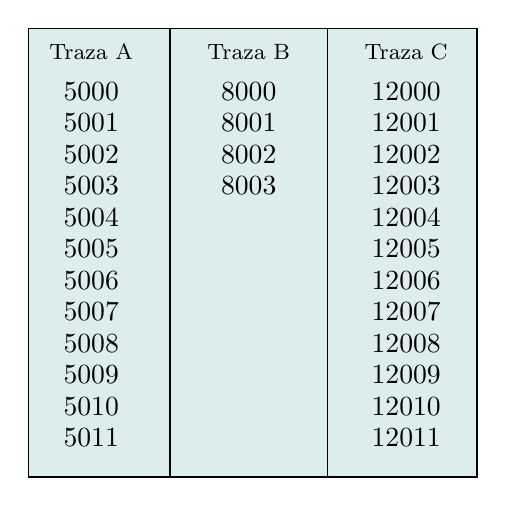
\begin{tikzpicture}
    \draw[fill=white!93!green!93!blue] (-.8,.4) rectangle (4.9,-5.3);
    \draw (1,.4) -- (1,-5.3);
    \draw (3,.4) -- (3,-5.3);
    \node[font=\footnotesize] at (0,.1) {Traza A};
    \node[font=\footnotesize] at (2,.1) {Traza B};
    \node[font=\footnotesize] at (4,.1) {Traza C};
    \def\y{0} 
    \foreach \i [remember=\y as \lasty (initially 0)] in {00,01,02,03,04,05,06,07,08,09,10,11} {
      \pgfmathsetmacro{\y}{\lasty - 0.4}
      \node at (0, \y) {50\i};
      \node at (4, \y) {120\i};
    }
    \def\y{0} 
    \foreach \i [remember=\y as \lasty (initially 0)] in {00,01,02,03} {
      \pgfmathsetmacro{\y}{\lasty - 0.4}
      \node at (2, \y) {80\i};
    }
  \end{tikzpicture}
  \caption{Traza de los procesos A, B y C.}
  \label{fig:traza_procesos}
\end{figure}

El sistema operativo aplica un quantum\footnote{Quantum: cantidad máxima de instrucciones (o, en general, de tiempo de CPU) que un proceso puede ejecutar antes de ser interrumpido por el planificador.} de 6 instrucciones, por lo que ningún proceso puede ejecutar más de seis instrucciones consecutivas antes de ser interrumpido. Inicialmente, el procesador ejecuta las seis primeras instrucciones del proceso A. Al agotarse el quantum, el dispatcher toma el control y transfiere la ejecución al proceso B.

El proceso B ejecuta cuatro instrucciones y, en la cuarta, solicita una operación de entrada/salida (E/S). Como debe esperar a que esta finalice, el proceso pasa al estado de espera y el procesador, mediante el dispatcher, continúa con el proceso C. Tras finalizar el quantum de C, el procesador vuelve a A. Cuando A vuelve a agotar su quantum, B todavía sigue esperando la finalización de la operación de E/S, por lo que el sistema operativo selecciona nuevamente al proceso C.

Este ejemplo muestra cómo, aunque cada proceso tiene su propia secuencia de ejecución, el procesador alterna entre ellos de acuerdo con la planificación del sistema operativo y con eventos como la expiración del quantum o la espera por operaciones de E/S.

\subsection{Modelo de dos estados}

\begin{figure}[!ht]
  \centering 
  \begin{tikzpicture}[>=Stealth]
    \node[
      draw,
      thin,
      minimum width=2.8cm,
      minimum height=1cm,
      shape=ellipse,
      inner sep=0pt,
      font=\small,
      text=black,
      outer color=white!85!green!85!blue,
      inner color=white,
    ] (nrun) {Not Running};

    \node[
      draw,
      thin,
      minimum width=2.8cm,
      minimum height=1cm,
      shape=ellipse,
      inner sep=0pt,
      font=\small,
      text=black,
      outer color=white!85!green!85!blue,
      inner color=white,
      right=2cm of nrun
    ] (run) {Running};
    \draw[->] (nrun.north) to[out=45, in=135] node[above,font=\footnotesize]{Dispatch} (run.north);
    \draw[->] (run.south) to[out=-135, in=-45] node[below,font=\footnotesize]{Pause} (nrun.south);
    \draw[<-] (nrun.west) -- node[above,font=\footnotesize]{Enter} ++(-2,0);
    \draw[->] (run.east) -- node[above,font=\footnotesize]{Exit} ++(2,0);
  \end{tikzpicture}
  \caption{Diagrama de transiciones de estados}
  \label{fig:two-state-model}
\end{figure}

La responsabilidad principal del sistema operativo es controlar la ejecución de los procesos, determinando cuándo se ejecutan y asignándoles los recursos necesarios. El modelo más simple para describir el comportamiento de un proceso considera únicamente dos estados posibles (Figura \ref{fig:two-state-model}):
\begin{itemize}
  \item \textbf{Running} (ejecutando): el proceso está siendo ejecutado por el procesador.
  \item \textbf{Not Running} (detenido): el proceso existe, pero no se encuentra ejecutándose.
\end{itemize}

Cuando el sistema operativo crea un nuevo proceso, genera su \emph{Process Control Block} (PCB) y lo incorpora al sistema en estado \emph{Not Running}. Posteriormente, el despachador (\emph{dispatcher}) selecciona uno de los procesos en espera para ejecutarlo, produciendo una transición al estado \emph{Running}. Del mismo modo, cuando el proceso en ejecución es interrumpido, vuelve al estado \emph{Not Running} y otro proceso ocupa el procesador.

Este modelo ya pone de manifiesto dos elementos fundamentales del sistema operativo. En primer lugar, cada proceso debe estar representado mediante un PCB que almacene su estado y toda la información necesaria para administrarlo. En segundo lugar, los procesos que no se están ejecutando deben mantenerse en una cola de espera como se muestra en la figura \ref{fig:queue_diagram_2_states} desde la cual el \emph{dispatcher} seleccionará el siguiente proceso a ejecutar. Si un proceso finaliza o es abortado, simplemente se elimina del sistema.

\begin{figure}[ht]
  \centering
  \includegraphics[width=0.7\textwidth]{chapters/02_unit/media/2state_diagram_queue.pdf}
  \caption{Diagrama de cola (queue).}
  \label{fig:queue_diagram_2_states}
\end{figure}

\subsection{Creación y terminación de procesos}

Todo proceso posee un ciclo de vida delimitado por su creación y su terminación.

\paragraph{Creación de procesos}

La creación de un proceso consiste en construir las estructuras de datos necesarias para administrarlo (principalmente su PCB) y reservar el espacio de memoria que utilizará durante su ejecución.

Las causas más habituales de creación de un proceso son:

\begin{itemize}
  \item Envío de un nuevo trabajo (\emph{batch job}).
  \item Inicio de sesión de un usuario en un sistema interactivo.
  \item Creación por parte del sistema operativo para proporcionar un servicio (por ejemplo, administrar una impresión).
  \item Creación por otro proceso (\emph{process spawning}).
\end{itemize}

En los sistemas modernos es frecuente que un proceso pueda crear otros procesos. El proceso original recibe el nombre de \textbf{proceso padre} (\emph{parent process}), mientras que el nuevo proceso se denomina \textbf{proceso hijo} (\emph{child process}). Esta técnica facilita la modularidad, el paralelismo y la implementación de servidores capaces de atender múltiples solicitudes simultáneamente.

\paragraph{Terminación de procesos}

Un proceso puede finalizar de forma normal cuando completa su ejecución y solicita al sistema operativo su terminación. En sistemas interactivos, esto suele ocurrir cuando el usuario cierra una aplicación o finaliza su sesión.

Además de la finalización normal, un proceso puede terminar debido a distintos errores o condiciones excepcionales. Entre las causas más comunes se encuentran:

\begin{itemize}
  \item Exceder el tiempo máximo de ejecución.
  \item Falta de memoria disponible.
  \item Violaciones de memoria o de protección.
  \item Errores aritméticos (por ejemplo, división por cero).
  \item Errores de entrada/salida.
  \item Ejecución de instrucciones inválidas o privilegiadas.
  \item Intervención del sistema operativo o del administrador.
  \item Terminación del proceso padre o solicitud explícita de este.
\end{itemize}
